\section{Simulation}
This section shows a simulation of our game done in ModelSim. It shows the proper functioning of \texttt{LIVES}. The \texttt{CLK\_SLOW} is set to 10ns and the \texttt{CLK\_FAST} to 0.1ns to correctly display the LEDs. To simulate the movement of the paddle, the clock of \texttt{MOVE\_LEFT} is set at 0.5 sec and the clock of \texttt{MOVE\_RIGHT} at 0.4 sec. \texttt{GAME\_STATE} is at game\_play. The simulation lasts 3 seconds. It behaves like expected. \\

\begin{figure}[H]
    \centering
    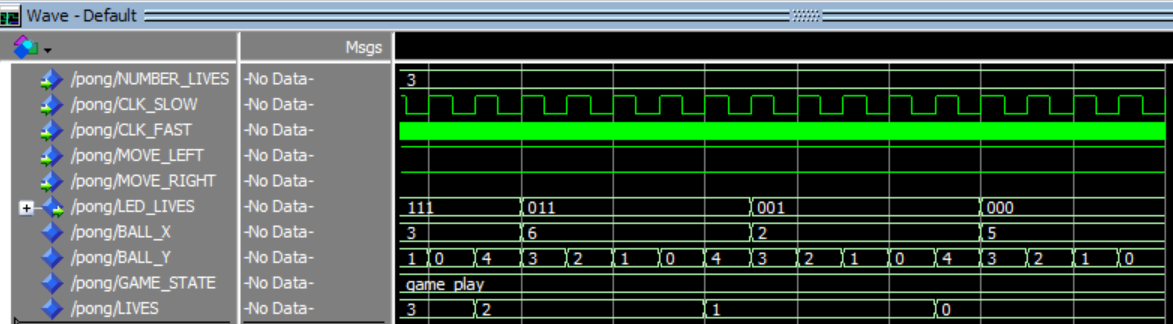
\includegraphics[scale = 0.3]{Ressources/png/simu.png}
    \caption{Simulation}
    \label{fig_2}
\end{figure}

It shows that \texttt{LIVES} decreases and that \texttt{LED\_LIVES} is correctly decremented. The \texttt{LIVES} go correctly from 3 to 0 and are decremented when \texttt{BALL\_Y} is at 0. \texttt{BALL\_X} is a random number and \texttt{BALL\_Y} is between 0 and 4. 